\lab{Спектральный анализ электрических сигналов}
\aim{изучить спектральный состав периодических электрических сигналов.}

\equip{анализатор спектра, генератор прямоугольных импульсов, генератор сигналов
специальной формы, осциллограф.}

Перед выполнением работы необходимо ознакомиться с теоретическим введением
к разделу.

В работе изучается спектральный состав периодических электрических сигналов
различной формы: последовательности прямоугольных импульсов, последовательности
цугов и амплитудно-модулированных гармонических колебаний. Спектры этих сигналов
наблюдаются с помощью анализатора спектра и сравниваются c рассчитанными
теоретически.

Периодическая функция может быть представлена в виде бесконечного ряда
гармонических функций --- ряда Фурье (см. п.~\ref{sec:spectrum-periodic}
Введения):
\[
f(t) = \sum_{n=-\infty}^{\infty} c_n e^{in\omega_0 t}\qquad\text{или}\qquad
f=\sum_{n=0}^{\infty} a_n \cos (n\omega_0 t + \varphi_n).
\]
Здесь $\omega_0 = 2\pi/T$, где $T$ --- период функции $f(t)$.
Коэффициенты $\{c_n\}$ могут быть найдены по формуле
\chaptereqref{coef-Fourier-periodic osc}:
\[
    c_n=\frac{1}{T}\int\limits_{0}^{T} f(t)e^{-in\omega_0 t}\,dt.
\]
Наборы коэффициентов разложения в комплексной $\{c_n\}$ и действительной
$\{a_n,\varphi_n\}$ формах связаны соотношением \chaptereqref{Fourier-coefficient}:
\[
a_n = 2|c_n|,\qquad \varphi_n = \arg c_n.
\]

\begin{wrapfigure}{o}{0.3\textwidth}
\centering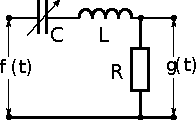
\includegraphics{Chapter_6/6-1-RLC.pdf}
\caption{Колебательный контур как узкополосный фильтр}
\figmark{simple-RLC}
\end{wrapfigure}

В качестве простейшего спектрального анализатора можно использовать
высокодобротный колебательный контур с подстраиваемой ёмкостью или
индуктивностью, рис.~\figref{simple-RLC}
(см. также п.~\ref{sec:spectrum-meaning} Введения).
Такой контур усиливает те гармоники входного сигнала $f(t)$,
частота которых близка к резонансной
$\nu_{рез} = 1/(2\pi\sqrt{LC})$, и практически не реагирует на частоты,
далёкие от $\nu_{рез}$. С точки зрения преобразования гармоник колебательный контур
является узкополосным \important{фильтром} с шириной полосы
пропускания порядка $\Delta \nu \sim \nu_{рез}/ Q$, где $Q =
\frac{1}{R}\sqrt{\frac{L}{C}} \gg 1$~--- его добротность. Амплитуда колебаний
в контуре пропорциональна амплитуде~$|c_n|$ гармоники $\nu_n=\nu_{рез}$
в фурье-спектре функции $f(t)$. Таким образом, меняя резонансную частоту контура
можно <<просканировать>> весь спектр.

\experiment

У описанной выше схемы есть существенный недостаток: при изменении~$L$ или~$C$
меняется также и добротность, а значит и ширина полосы пропускания.
Кроме того, изготовление настраиваемых контуров с высокой добротностью
непрактично. В~связи с этим, как правило, для фильтрации сигнала
применяется другая схема.

Исследуемый сигнал $f(t)$ и сигнал от вспомогательного генератора гармонических
колебаний частоте~$\nu_{гет}$ (генератор в таких схемах называют
\important{гетеродином}) подаются на вход \important{смесителя}. Смеситель
представляет собой нелинейный элемент, который из колебаний с частотами~$\nu_1$
и~$\nu_2$ на выходе генерирует сигналы на \emph{комбинированных}
частотах: $\nu_1 + \nu_2$ и $\nu_1 - \nu_2$.
<<Разностный>> сигнал смесителя поступает на фильтр ---
высокодобротный колебательный контур, настроенный на некоторую \emph{фиксированную}
резонансную частоту~$\nu_0$. Таким образом, если $f(t)$ содержит гармонику
$\nu_n=\nu_{гет}-\nu_0$, она будет усилена, а отклик будет
пропорционален её амплитуде.

Отметим, что смешение частот исследуемого сигнала и частоты гетеродина лежит в
основе большинства современных радиоприёмных устройств~---
\emph{супергетеродинов}.

\begin{figure}[h!]
\hfil
\pic{0.9\textwidth}{Chapter_6/6_1_1}
\caption{Структурная схема анализатора спектра}
\figmark{Spectrum analyzer}
\end{figure}

В спектральном анализаторе частота гетеродина пропорциональна напряжению,
подаваемому на развертку по оси~$X$ встроенного в анализатор осциллографа.
Выходной сигнал подаётся на канал~$Y$. На экране анализатора возникает, таким
образом, график, изображающий зависимость амплитуды гармоник исходного сигнала
от частоты, т.\,е. его спектр (заметим, что информация о фазах гармоник при этом
теряется).


\begin{lab:task}

\tasksection{А. Исследование спектра периодической последовательности прямоугольных
импульсов}

% \begin{figure}[h!]
% \centering
% \pic{0.9\textwidth}{6_1_2}
% \caption{Схема для исследования спектра периодической последовательности
% прямоугольных импульсов}
% \figmark{Scheme for square pulses}
% \end{figure}
%
% Схема для исследования спектра периодической последовательности прямоугольных
% импульсов представлена на рис.~\figref{Scheme for square pulses}.
%
% Сигнал с~выхода генератора прямоугольных импульсов Г5-54 подаётся на вход
% анализатора спектра и одновременно~--- на вход~$Y$ осциллографа. С~генератора
% импульсов на осциллограф подаётся также сигнал синхронизации, запускающий ждущую
% развёртку осциллографа. При этом на экране осциллографа можно наблюдать саму
% последовательность прямоугольных импульсов, а на экране ЭЛТ анализатора
% спектра~--- распределение амплитуд спектральных составляющих этой
% последовательности.
%
% В наблюдаемом спектре отсутствует информация об амплитуде нулевой гармоники,
% т.е. о~величине постоянной составляющей; её местоположение (начало отсчёта шкалы
% частот) отмечено небольшим вертикальным выбросом.

В этом упражнении исследуется зависимость ширины спектра $\Delta \nu$
периодической последовательности прямоугольных импульсов
от длительности отдельного импульса $\tau$.

\begin{figure}[h!]
\hfil\hfil
\begin{minipage}{0.4\textwidth}
    \pic{0.5\textwidth}{Chapter_6/6-1-imp}
    \caption{Периодическая последовательность импульсов}
\end{minipage}
\hfil
\begin{minipage}{0.4\textwidth}
% \begin{figure}
    \pic{0.5\textwidth}{Chapter_6/6-1-imps}
    \caption{Спектр последовательности импульсов}
\end{minipage}
\end{figure}

\begin{enumerate}

\item Ознакомьтесь с устройством приборов (генератор прямоугольных импульсов,
осциллограф, анализатор спектра) и подготовьте их к работе,
следуя техническим описаниям, расположенным на установке.

\item Подключите генератор прямоугольных импульсов через разветвитель
к осциллографу и анализатору спектра.

\item На генераторе задайте частоту повторения импульсов
$\nu_{повт} = 1\;кГц$ (период $T=1\;мс$), длительность импульса
$\tau=50\;мкс$. Получите устойчивую картину сигнала на осциллографе.

\item Предварительно оцените характерную ширину спектра
из соотношения неопределённостей $\Delta \nu \sim 1/\tau$
(см.  п.~\ref{sec:indeterminacy} Введения).

\item Получите спектр сигнала на анализаторе спектра. Предварительно
подберите начало отсчёта и диапазон измерения по частоте,
так чтобы на экране помещалась б\'{о}льшая часть спектра.

\item Измеяя параметры сигнала ($\nu_{повт}$, $\tau$),
наблюдайте, как изменяется его спектр. Опишите результаты.
Сфотографируйте или скопируйте на кальку несколько огибающих спектров
с различными параметрами, например:
а)~$\nu_{повт}=1\;кГц$, $\tau=50\;мкс$,
б)~$\nu_{повт}=1\;кГц$, $\tau=100\;мкс$,
в)~$\nu_{повт}=2\;кГц$, $\tau=50\;мкс$.
при фиксированном масштабе частот (по оси $X$) анализатора спектра [кГц/дел],
Параметры запишите в тетради, фотографии или кальку приложите к отчёту.
.

\item Проведите измерения зависимости ширины спектра от длительности
импульса~$\Delta \nu(\tau)$ при изменении $\tau$ от 25 до 200~мкс при
$\nu_\text{повт}=1$~кГц. Ширину определяйте по положению первой гармоники
с нулевой амплитудой.

\item Постройте график зависимости ширины спектра от обратного времени импусльа
$\Delta \nu(1/\tau)$ и по его наклону убедитесь в справедливости соотношения
неопределённостей. Оцените погрешность данного опыта.

\item Для одного из сигналов, наблюдаемых в п.~6, рассчитайте теоретические
значения амплитуд спектральных компонент по формуле \chaptereqref{impulses-spectrum}.
Сравните измеренные значения с теоретическими, изобразив их на одном графике.
\todo[inline]{Ссылка на пункт задания не автоматическая!}

\end{enumerate}


\tasksection{Б. Исследование спектра периодической~последовательности цугов
гармонических~колебаний}

В этом упражнении исследуется зависимость расстояния между ближайшими
спектральными компонентами от частоты повторения цугов.

\begin{figure}[h!]
\hfil\hfil
\begin{minipage}{0.4\textwidth}
    \pic{0.5\textwidth}{Chapter_6/v6-zug}
    \caption{Периодическая последовательность цугов}
\end{minipage}
\hfil
\begin{minipage}{0.4\textwidth}
% \begin{figure}
    \pic{0.5\textwidth}{Chapter_6/6-1-zugs}
    \caption{Спектр последовательности цугов}
\end{minipage}
\end{figure}


\begin{enumerate}

\item По техническому описанию к работе соберите схему, используемую
для генерации последовательности синусоидальных цугов.

\item Установите частоту несущей $\nu_0=25$~кГц и получите на экране осциллографа
устойчивую картину цугов.

\item Получите спектр сигнала. Наблюдайте, как изменяется вид спектра:
а)~при увеличении длительности импульса (например, $\tau=50$, $100$~мкс
для $\nu_\text{повт}=1\;кГц$); б)~при изменении частоты несущей:
$\nu_0=25$,~10 или~40~кГц; в)~при изменении частоты повторения
$\nu_{повт}=1,\;2$~кГц. Опишите результаты или зарисуйте качественную
картину в~тетради.

\item При фиксированной длительности импульсов $\tau=50$~мкс исследуйте
зависимость расстояния~$\delta \nu$ между соседними спектральными компонентами
периода повторения импульсов $T=1/\nu_\text{повт}$
(в~диапазоне частот 1--8~кГц).

\item Постройте график $\delta \nu(1/T)$ и по его наклону
убедитесь в~справедливости соотношения неопределённости.
Оцените погрешность данного опыта.

% \item Сравните зарисованные на кальку спектры:
% \begin{itemize}
% 	\item прямоугольных импульсов при одинаковых периодах и разных
% длительностях импульса $\tau$;
% 	\item цугов при одинаковых $\tau$ и разных периодах;
% 	\item цугов и прямоугольных импульсов при одинаковых значениях~$\tau$
% и~$T$.
% \end{itemize}
\end{enumerate}

\tasksection{В. Исследование спектра гармонических сигналов, модулированных по
амплитуде}

%\eo Схема для исследования амплитудно-модулированного сигнала представлена на
% \p{4}.
% Модуляционный генератор встроен в~левую часть генератора сигналов Г6-34 .
% Синусоидальный сигнал с~частотой модуляции $f_{мод}=1$~кГц подаётся
% с~модуляционного генератора на вход АМ (амплитудная модуляция) генератора,
% вырабатывающего синусоидальный сигнал высокой частоты (частота
% несущей~$\nu_0=25$~кГц). Амплитудно-модулированный сигнал с~основного выхода
% генератора поступает на осциллограф и на анализатор спектра.

% \begin{figure}[h!]
% \centering
% \pic{0.9\textwidth}{6_1_4}
% \caption{Схема для исследования спектра высокочастотного гармонического
% сигнала, промодулированного по~амплитуде низкочастотным гармоническим~сигналом}
% \figmark{Scheme for amplitude modulation}
% \end{figure}

В этом упражнении исследуется зависимость отношения амплитуд спектральных линий
синусоидального сигнала, модулированного низкочастотными гармоническими
колебаниями, от коэффициента модуляции, измеряемого с~помощью осциллографа.

\begin{figure}[h!]
\hfil\hfil
\begin{minipage}{0.4\textwidth}
    \pic{0.5\textwidth}{Chapter_6/6-1-mod}
    \caption{Модулированный по амплитуде сигнал}
\end{minipage}
\hfil
\begin{minipage}{0.4\textwidth}
    \pic{0.5\textwidth}{Chapter_6/6-1-mods}
    \caption{Спектр модулированного сигнала}
\end{minipage}
\end{figure}
\todo[inline]{Выровнять рисунки}

\begin{enumerate}
\item Следуя техническому описанию на установке соберите схему для
генерации гармонических модулированных колебаний.

\item Установите частоту несущей $\nu_0=25\;кГц$, частоту модуляции
$\nu_{мод} = 1\;кГц$ и глубину модуляции $m=1$.
Получите на экране осциллографа устойчивую картину.

\item Получите спектр исследуемого сигнала. Измерьте положения центральной
и боковой гармоник. Изменяя частоту модулирующего сигнала $\nu_{мод}$
и частоту несущей $\nu_0$, наблюдайте, как измеяется положение спектральных линий.
Опишите или зарисуйте результат в тетрадь.

\item Меняя глубину модуляции~$m$, измеряйте отношение амплитуд
боковой и основной линий спектра $\frac{a_\text{бок}}{a_\text{осн}}$
в зависимости от~$m$;
для расчёта глубины модуляции~$m$ используйте формулу \chaptereqref{modul-deep}:
\[
    m = \frac{A_{\rm max} - A_{\rm min}}{A_{\rm max} + A_{\rm min}},
\]
где максимальная~$A_{\rm max}$ и минимальная~$A_{\rm min}$ амплитуды сигнала
измеряются с помощью осциллографа.

\item Постройте график отношения $a_\text{бок}/a_\text{осн}$
в~зависимости от~$m$. Определите угол наклона графика и сравните
с результатами п.~\ref{sec:modulated-spectrum}. Оцените погрешность данного опыта.
\end{enumerate}

\end{lab:task}



%\lit

%\n \emph{Сивухин Д.В.} Общий курс физики. Т.~III. Электричество~--- М.: Наука,
% 1983. \S~128.

%\n \emph{Крауфорд Ф.} Берклеевский курс физики. Т.~III. Волны.~--- М.: Наука,
% 1976. \S~6.4.
